%%%%%%%%%%%%%%%%%%%%%%%%%%%%%%%%%%%%%
%                                   %
% Compile with XeLaTeX and biber    %
%                                   %
% Questions or comments:            %
%                                   %
% joshua dot mcneill at uga dot edu %
%                                   %
%%%%%%%%%%%%%%%%%%%%%%%%%%%%%%%%%%%%%

\documentclass{beamer}
  % Read in standard preamble (cosmetic stuff)
  %%%%%%%%%%%%%%%%%%%%%%%%%%%%%%%%%%%%%%%%%%%%%%%%%%%%%%%%%%%%%%%%
% This is a standard preamble used in for all slide documents. %
% It basically contains cosmetic settings.                     %
%                                                              %
% Joshua McNeill                                               %
% joshua dot mcneill at uga dot edu                            %
%%%%%%%%%%%%%%%%%%%%%%%%%%%%%%%%%%%%%%%%%%%%%%%%%%%%%%%%%%%%%%%%

% Beamer settings
% \usetheme{Berkeley}
\usetheme{CambridgeUS}
% \usecolortheme{dove}
% \usecolortheme{rose}
\usecolortheme{seagull}
\usefonttheme{professionalfonts}
\usefonttheme{serif}
\setbeamertemplate{bibliography item}{}

% Packages and settings
\usepackage{fontspec}
  \setmainfont{Charis SIL}
\usepackage{hyperref}
  \hypersetup{colorlinks=true,
              allcolors=blue}
\usepackage{graphicx}
  \graphicspath{{../../figures/}}
\usepackage[normalem]{ulem}
\usepackage{enumerate}

% Document information
\author{M. McNeill}
\title[FREN2001]{Français 2001}
\institute{\url{joshua.mcneill@uga.edu}}
\date{}

%% Custom commands
% Lexical items
\newcommand{\lexi}[1]{\textit{#1}}
% Gloss
\newcommand{\gloss}[1]{`#1'}
\newcommand{\tinygloss}[1]{{\tiny`#1'}}
% Orthographic representations
\newcommand{\orth}[1]{$\langle$#1$\rangle$}
% Utterances (pragmatics)
\newcommand{\uttr}[1]{`#1'}
% Sentences (pragmatics)
\newcommand{\sent}[1]{\textit{#1}}
% Base dir for definitions
\newcommand{\defs}{../definitions}


  % Packages and settings

  % Document information
  \subtitle[Sites et \lexi{où} et \lexi{qui}]{Les sites et les relatifs \lexi{où} et \lexi{qui}}

\begin{document}
  % Read in the standard intro slides (title page and table of contents)
  \begin{frame}
    \titlepage
    \tiny{Office: % Basically a variable for office hours location
Gilbert 121\\
          Office hours: % Basically a variable for office hours
 lundi, mercredi, vendredi 10:10--11:10
}
  \end{frame}

  \begin{frame}[t]{Décrivons-les}
    \begin{columns}
      \column{0.5\textwidth}
        Décrivons les endroits suivants en utilisant des pronoms relatifs.
        \begin{enumerate}
          \item C'est une cave où/qui ...
          \item<2-> C'est un village médiéval où/qui ...
          \item<3-> C'est une abbaye où/qui ...
          \item<4-> C'est un théâtre romain où/qui ...
          \item<5-> C'est une cuisine où/qui ...
        \end{enumerate}
      \column{0.5\textwidth}
        \begin{minipage}[c][0.8\textheight]{\linewidth}
          \begin{center}
            \only<1>{
              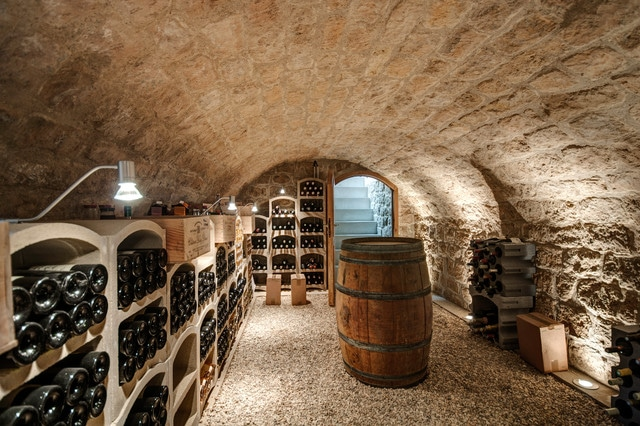
\includegraphics[scale=0.25]{cave.jpg}
            }
            \only<2>{
              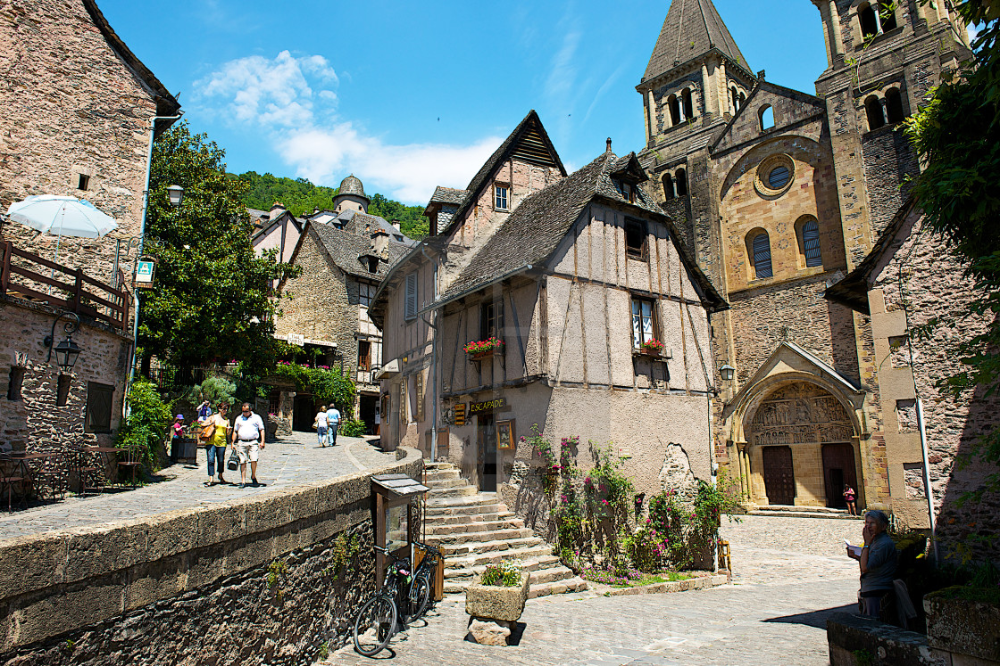
\includegraphics[scale=0.16]{village_médiéval.png} \\
              Conques, France
            }
            \only<3>{
              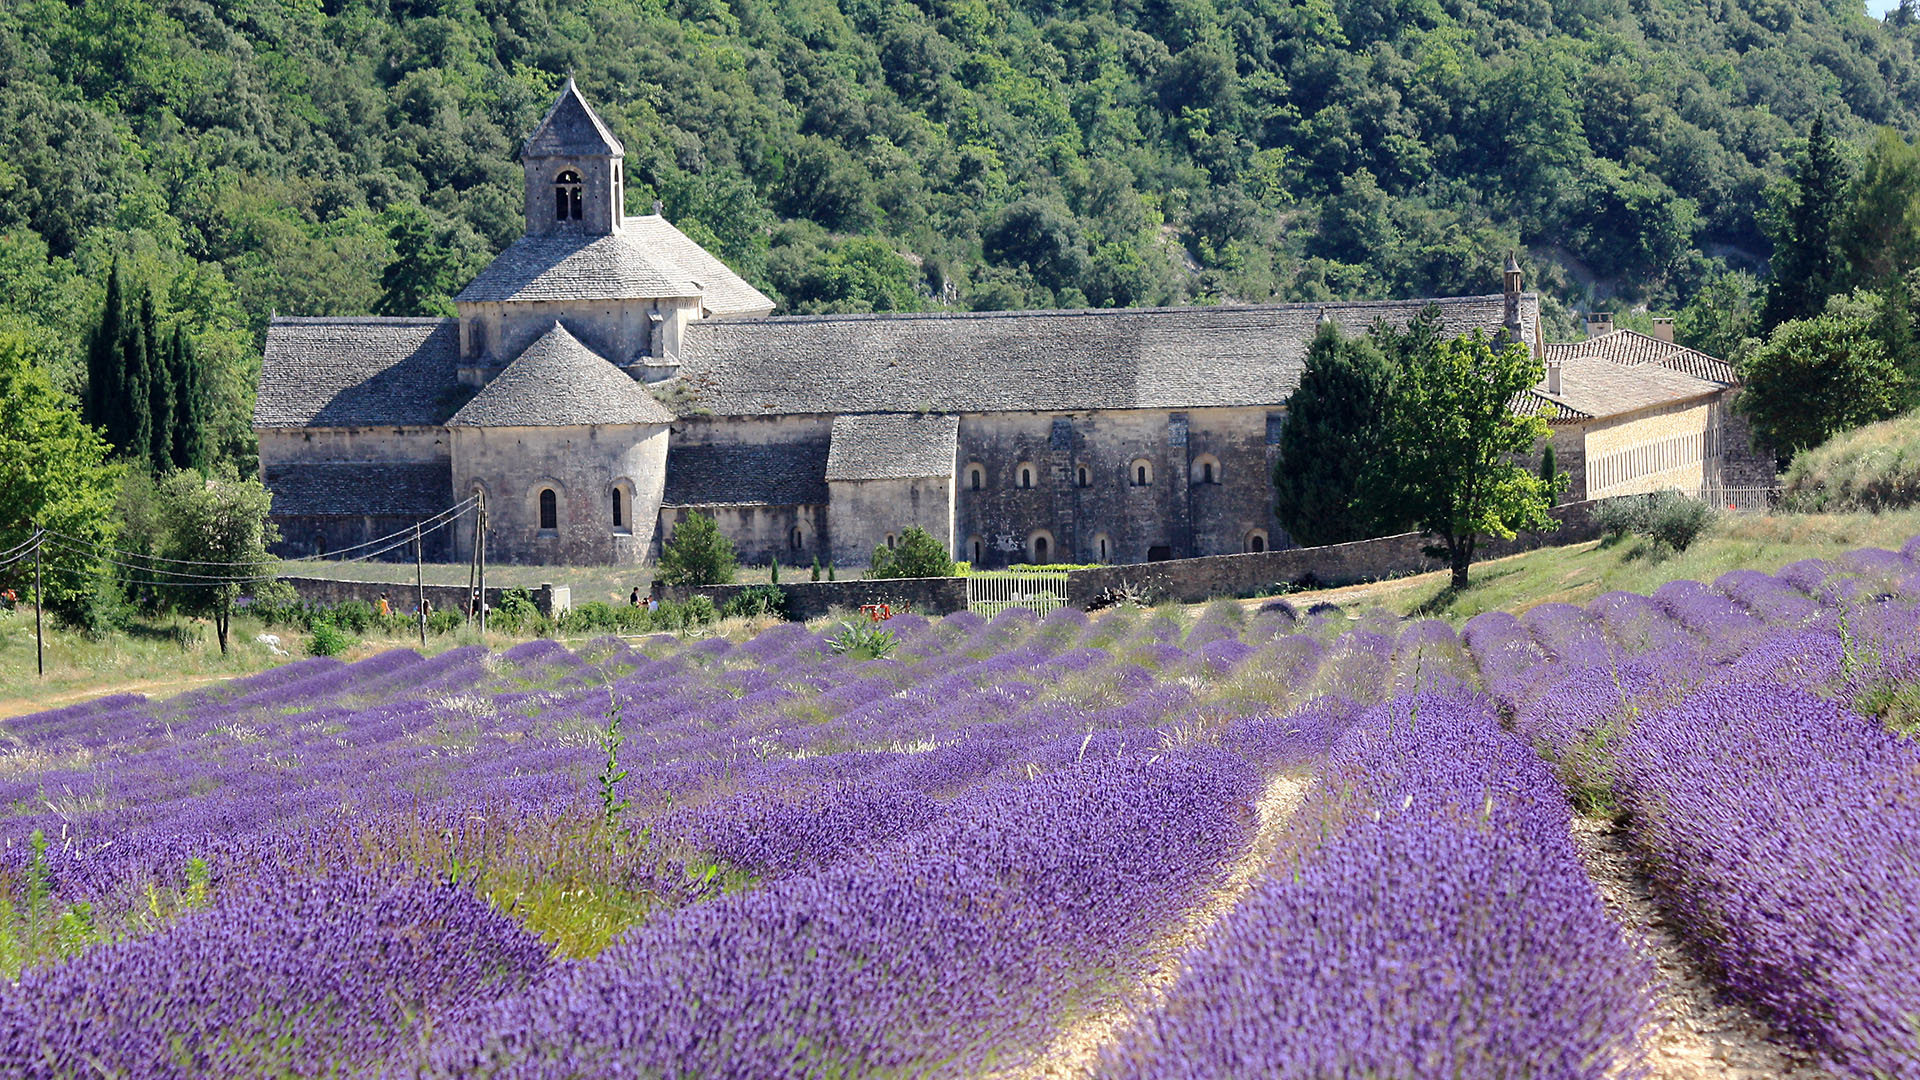
\includegraphics[scale=0.22]{abbaye.jpg} \\
              L'abbaye Notre-Dame de Sénanque
            }
            \only<4>{
              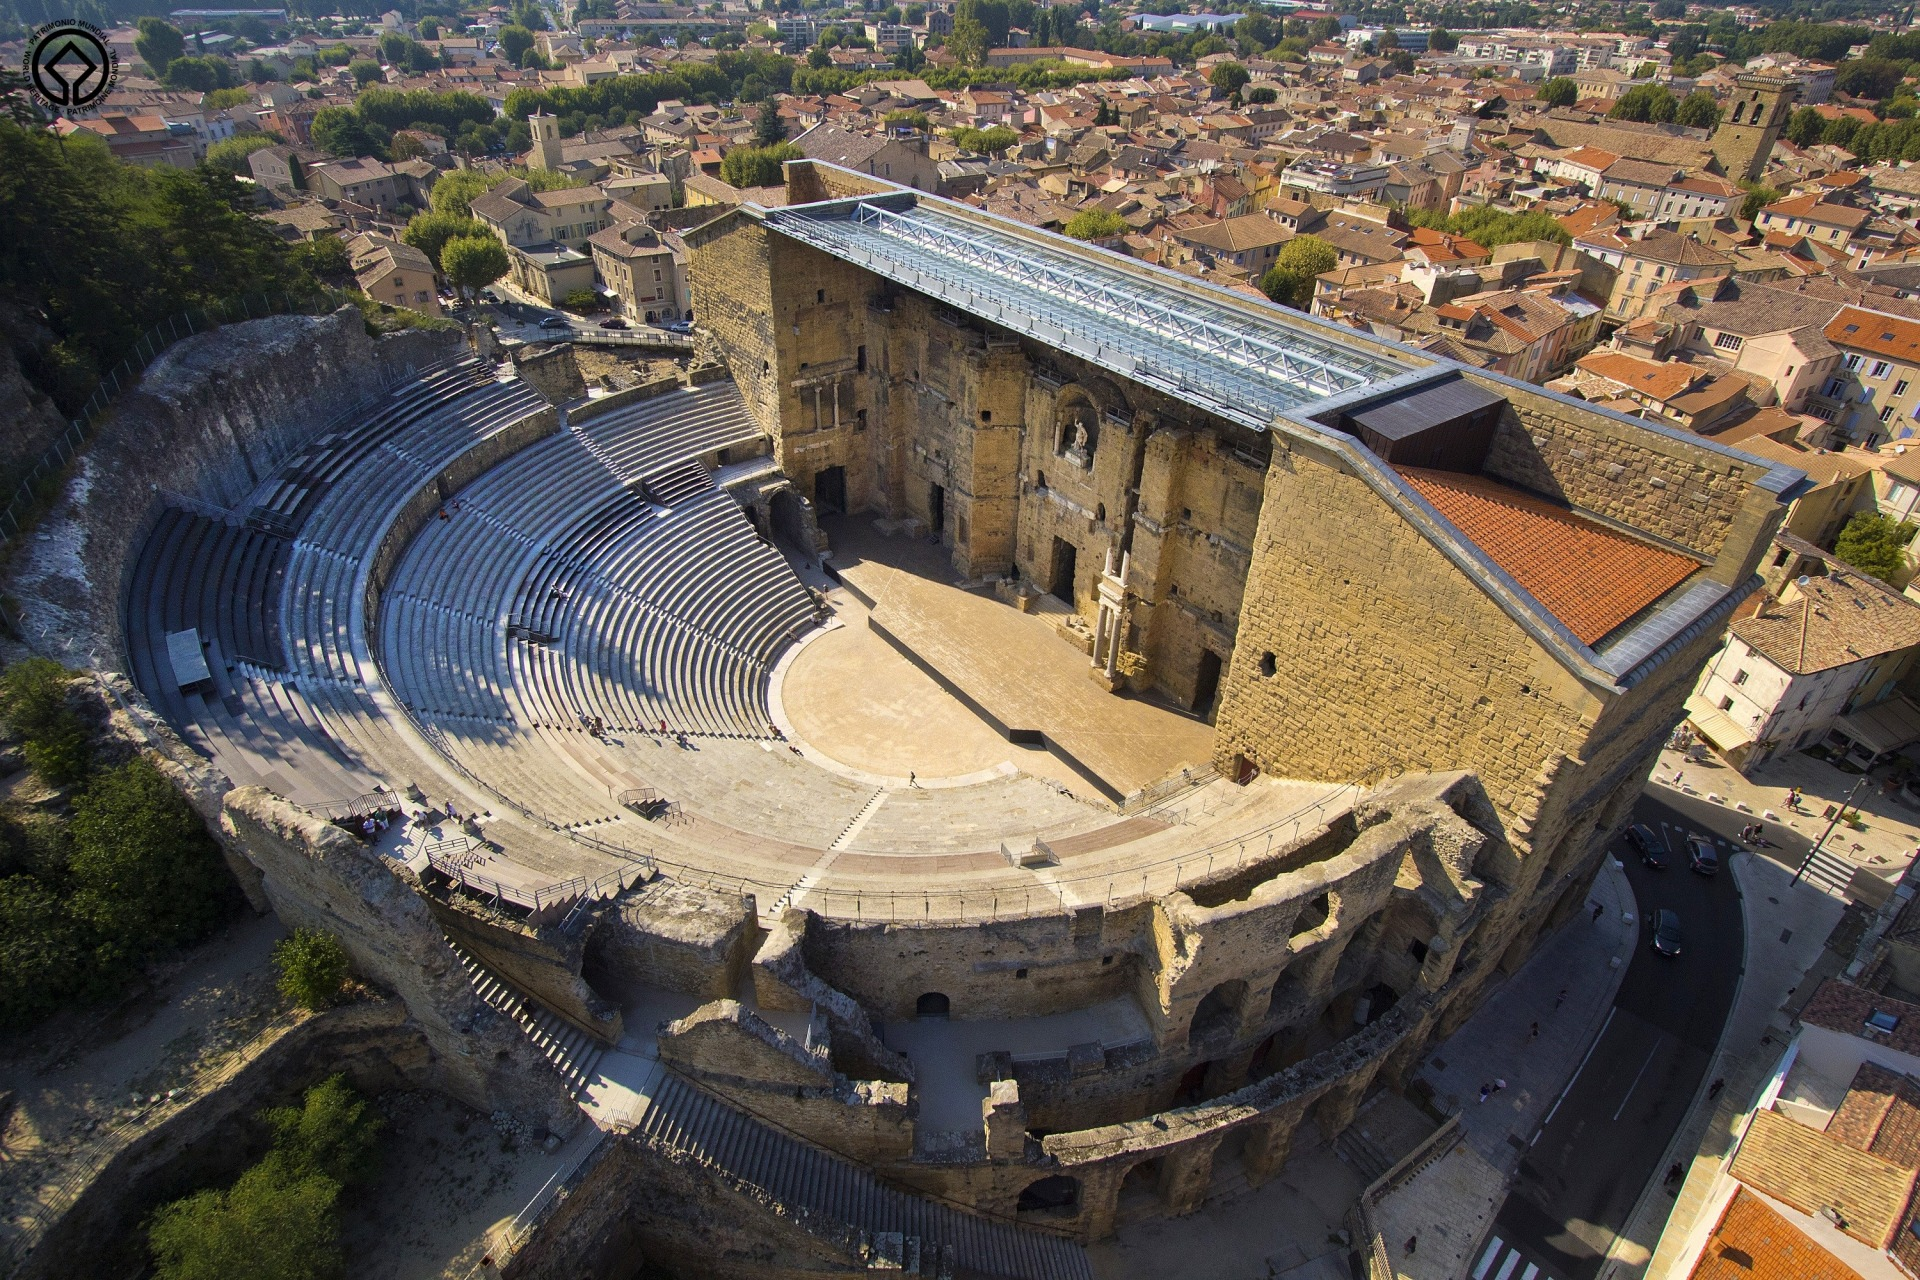
\includegraphics[scale=0.11]{théâtre_romain.jpg}
              Théâtre antique d'Orange
            }
            \only<5>{
              
\includegraphics[scale=0.25]{cuisine.jpg}
            }
          \end{center}
        \end{minipage}
    \end{columns}
  \end{frame}

  \begin{frame}{}
    \begin{center}
      \Large Quiz
    \end{center}
  \end{frame}

  \begin{frame}{}
    Demande à un/e partenaire s'il ou si elle va aux endroits suivants.
    Il/Elle doit te donner une raison pourquoi.
    \alert{N'oublie pas} d'utiliser le pronom \alert{y} dans tes réponses!
    \begin{columns}[t]
      \column{0.6\textwidth}
        \begin{description}
          \item[] \textbf{Modèle:} \textit{dans des bons restaurants}
          \item[E1:] Tu vas quelquefois dans des bons restaurants?
          \item[E2:] Non, je n'\alert{y} vais jamais.
          \item[E1:] Pourquoi?
          \item[E2:] Parce qu'ils sont très chers, et je n'ai pas assez d'argent pour \alert{y} aller.
        \end{description}
      \column{0.4\textwidth}
        \begin{enumerate}
          \item au théâtre
          \item à des concerts
          \item dans un café
          \item au musée
          \item à la plage
          \item à la montagne
          \item en Europe
          \item dans un pays francophone
        \end{enumerate}
    \end{columns}
  \end{frame}

  \begin{frame}{Un endroit logique}
    \small
    Avec un/e partenaire, propose des endroits logiques pour chaque \alert{y}.
    \begin{description}
      \item[] \textbf{Modèle:} \textit{Nous y sommes allés pour bronzer et faire de la plongée au bord de la mer.}
      \item[E1\&E2:] En Guadeloupe ou à la plage ou dans la Côte d'Azur ou ...
    \end{description}
    \begin{columns}[t]
      \column{0.5\textwidth}
        \begin{enumerate}
          \item On va y aller pour faire du ski et de la motoneige.
          \item Les Marchand y ont fait un tour à vélo.
          \item On y passe les vacances à bord d'un bateau à voile.
        \end{enumerate}
      \column{0.5\textwidth}
        \begin{enumerate}
          \setcounter{enumi}{3}
          \item Christian va y passer ses vacances pour économiser \gloss{save} son argent.
          \item Nous y avons pris un petit avion pour survoler \gloss{fly over} les îles.
          \item J'y suis allé avec des copains pour faire du camping et de la randonnée.
        \end{enumerate}
    \end{columns}
  \end{frame}

  \begin{frame}{}
    \begin{center}
      \Large Questions?
    \end{center}
  \end{frame}
\end{document}
